%!TEX root = ../../main.tex


\subsection{Struktur}
\frame{
	\frametitle{Was gehört dazu?}

	\begin{description}
		\item [Feature Selection] Welche Punkte sind \textit{repräsentativ} für das Objekt/die Szene?
		\item [1. Reference Frame/Axis] Welche \textit{Referenz} wird für die Nachbarschaft gewählt
		\item [2. Histogramm/Signatur] Welche \textit{Berechnungsvorschrift} wird ausgeführt?
		\item [3. Matching-Phase] Wie werden berechnete Deskriptoren verglichen?
	\end{description}


	    \begin{figure}
        \centering
        \begin{subfigure}[b]{0.35\textwidth}
            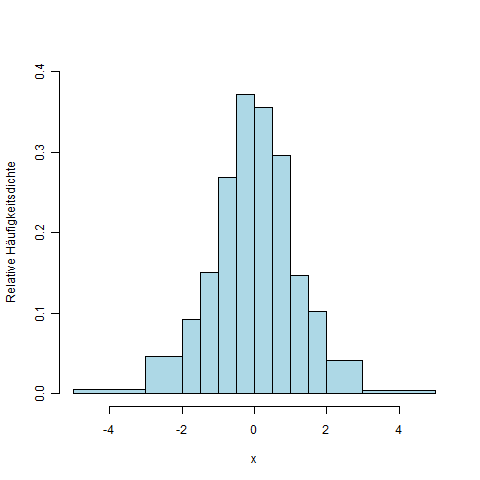
\includegraphics[width=\textwidth]{topics/eigenschaften/hist.png}
            \caption{Histogramm}
            \label{fig:hist}
        \end{subfigure}
        ~~~
        \begin{subfigure}[b]{0.35\textwidth}
            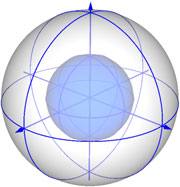
\includegraphics[width=\textwidth]{topics/intro/n3d.png}
            \caption{3D-Nachbarschaft}
            \label{fig:ctKnut}
        \end{subfigure}
    \end{figure}


}
\subsection{Schwierigkeiten}
\frame{
	\frametitle{Was sind die Schwierigkeiten?}

	\begin{flushleft}
	\setbeamertemplate{description item}[align left]
	\begin{description}
		\item[Geometrische Transformationen] Rotation und Translation sollen möglichst geringen Einfluss auf das Ergebnis haben.
		\item[Skalierung] Ein in der größe skaliertes Objekt soll die selbe Deskription erhalten.
		\item[Punktdichte] Unterschiedliche Sensoren und Blickwinkel führen zu Schankungen.
		\item[Clutter] Viele Objekte, ein Durcheinander
		\item[Verdeckung] Objekte verdecken andere
		\item[Vorzeichen] Eindeutigkeit des Referenzsystems.
	\end{description}
	\end{flushleft}
}